\chapter{環境構築}
\label{chap:chap01-install}

各種アルゴリズムの説明に入る前に、今回作成するWebアプリの基本構成および環境構築の方法について説明します。

各章でそれぞれ一つのミニアプリを作る予定ですが、すべて同じ環境上に作るため、ここでまとめて説明します。

\section{今回の構成}
\label{sec:1-1}

今回は以下の構成でWebアプリを作ります。

\begin{reviewimage}%%architecture
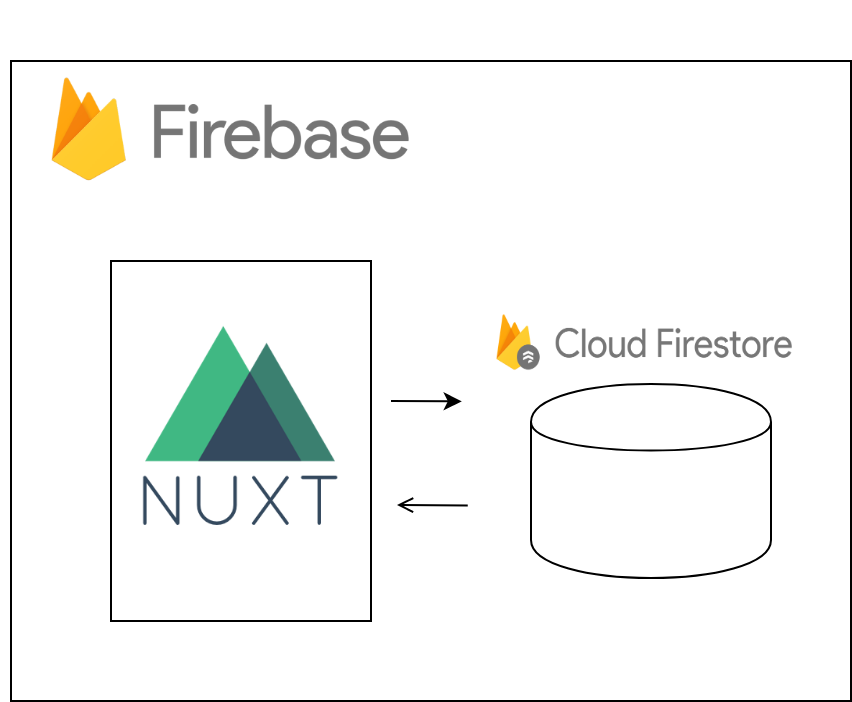
\includegraphics[width=\maxwidth]{./images/architecture.png}%
\reviewimagecaption{今回の構成}
\label{image:chap01-install:architecture}
\end{reviewimage}

それぞれの要素について説明します。

\subsection*{Firebase}
\addcontentsline{toc}{subsection}{Firebase}
\label{sec:1-1-1}

今回は、Firebaseと呼ばれるWebサイトのホスティングやDBをサクッと作れるBaaS(Backend as a service)上にWebサービスを作ります。
Firebaseを利用することで、難しかったインフラ構築やサーバーデプロイなどの作業が不要になるため、一人でWebサービスをサクッとプロトタイピングするのに向いています。

サクッと一人で、コストも抑えてWebアプリを作るため、Firebaseを今回は採用することにしました。

\subsection*{Firebase Hosting}
\addcontentsline{toc}{subsection}{Firebase Hosting}
\label{sec:1-1-2}

Firebase HostingはFirebaseのサービスの一つで、HTMLやCSS、JSなどの静的ファイルをホスティングするためのサービスです。
PHPやJava, Pythonなどはもちろん動きませんが、後述する「静的サイトジェネレーター」を組み合わせることで、フロントエンドフレームワークで作成された
ファイルをデプロイすることができます。

コストも抑えることができるので、個人開発などにおすすめです。

\subsection*{Cloud Firestore}
\addcontentsline{toc}{subsection}{Cloud Firestore}
\label{sec:1-1-3}

データの永続化を行うDBです。少し前のWebサービスだと \texttt{MySQL}や」

\subsection*{Nuxt.js}
\addcontentsline{toc}{subsection}{Nuxt.js}
\label{sec:1-1-4}

今回、Nuxt.jsと呼ばれるフロントエンドフレームワークを用いて、Webサービスを作成します。Nuxt.jsはVue.jsと呼ばれるフレームワークはベースになっており
HTML/CSSが理解できていれば、非常に理解しやすく扱いやすいフロントエンドフレームワークです。

Nuxt.jsには「静的サイトジェネレーター」の機能もあり、これを用いて、生成されたHTML/CSSなどを firebase hostingにデプロイすることで
今回のWebアプリを作っていきます。

\subsection*{Cloud Firestore}
\addcontentsline{toc}{subsection}{Cloud Firestore}
\label{sec:1-1-5}

\section{環境をつくろう}
\label{sec:1-2}

\subsection*{Firebaseへのサインアップ}
\addcontentsline{toc}{subsection}{Firebaseへのサインアップ}
\label{sec:1-2-1}

\subsection*{Nuxt.jsの導入}
\addcontentsline{toc}{subsection}{Nuxt.jsの導入}
\label{sec:1-2-2}
